\documentclass[12pt]{article}
\usepackage[utf8]{inputenc}
\usepackage{amsmath}
\usepackage{amsfonts}
\usepackage{amssymb}
\usepackage{empheq}
\usepackage{tikz}
\usepackage{changepage}
\usetikzlibrary{automata, positioning, shapes, arrows}
\addtolength{\topmargin}{-0.875in}
\addtolength{\textheight}{1.75in}

\title{Regarding Positive Even Zeta Values}
\author{Ethan Jensen}
\date{January 1, 2019}

\begin{document}
	\maketitle
	\tikzset{
		->, % makes the edges directed
		>=triangle 45, % makes the arrow heads bold
		node distance=3cm, % specifies the minimum distance between two nodes. Change if necessary.
		every state/.style={thick, fill=gray!10}, % sets the properties for each ’state’ node
		initial text=$ $, % sets the text that appears on the start arrow
	}
\definecolor{mycolor1}{RGB}{230,230,230}
\definecolor{mycolor2}{RGB}{210,210,210}
\definecolor{mycolor3}{RGB}{190,190,190}
\section{Condition codes}
\noindent
Recall that \(\mathbb{Z}_+^n\) is defined as
\[\mathbb{Z}_+^n=\{(x_1,x_2,...x_n)|x_1,x_2,...x_n\in\mathbb{Z}_+\}\]
We can define a disjoint partition on \(\mathbb{Z}_+^n\) into subsets based on how elements of the tuple \((x_1,x_2,...x_n)\) are equal to each other.
\newline \newline
\textbf{Definition 1.1.} \textit{Let S be a set of tuples. A \textbf{condition code} C on S is a tuple} \((c_1, c_2,...c_n)\) \textit{that gives S the following elementhood condition:} \newline
\begin{adjustwidth}{2.5em}{0pt}
	\textit{A tuple x is an element of S if and only if there exists a tuple t = \((t_1,t_2,...t_n) \in \mathbb{Z}_+^n\) such that for all i, x contains \(c_i\) copies of \(t_i\).}
\end{adjustwidth}
\(\ \)
\newline
\textbf{Definition 1.2.} \textit{A condition code C is \textbf{spicy} if it gives the following two elementhood conditions:}
\begin{adjustwidth}{2.5em}{0pt}
	\textit{\textbf{(a)} A tuple x is an element of S if and only if there exists a tuple t = \((t_1,t_2,...t_n) \in \mathbb{Z}_+^n\) such that for all i, x contains \(c_i\) copies of \(t_i\).}
	\newline
	\newline
 \textbf{(b) } \textit{Each }\(t_i\)\textit{ is distinct.}
\end{adjustwidth}
\textit{A condition code C that is not spicy is called }\textbf{mild}
\newline
\newline
\textbf{Definition 1.4.} \textit{A condition code C is \textbf{super spicy} if it gives the following two elementhood conditions:}
\begin{adjustwidth}{2.5em}{0pt}
	\textit{\textbf{(a)} A tuple x is an element of S if and only if there exists a tuple t = \((t_1,t_2,...t_n) \in \mathbb{Z}_+^n\) such that for all i, x contains \(c_i\) copies of \(t_i\).}
	\newline
	\newline
 \textbf{(b) } \(t_i < t_{i+1}\) if \(c_i = c_{i+1}\) \textit{ and } \(t_i \neq t_{i+1}\) \textit{ if } \(c_i \neq c_{i+1}\)
\end{adjustwidth}
\(\ \)
\newline
\textbf{Definition 1.4.}
\begin{adjustwidth}{2.5em}{0pt}
	\textbf{(a)}\textit{ A \textbf{mild subset} S of }\(\mathbb{Z}_n^+\)\textit{ written }\(S(c_1)(c_2)...(c_k)\) \textit{ is a subset of }\(\mathbb{Z}_n^+\) \textit{ whose only restrictions on elementhood is a mild condition code.}
	\newline
	\textbf{(b)}\textit{ A \textbf{spicy subset} S of }\(\mathbb{Z}_n^+\)\textit{ written }\(S(c_1,c_2,...c_k)\) \textit{ is a subset of }\(\mathbb{Z}_n^+\) \textit{ whose only restrictions on elementhood is a spicy condition code. S can be identified as a subset of a unique mild subset S'.}
	\newline
	\textbf{(c)}\textit{ A \textbf{super spicy subset} S of \(\mathbb{Z}_n^+\)\textit{ written the same as a spicy subset is a subset of }\(\mathbb{Z}_n^+\) \textit{ whose only restrictions on elementhood is a super spicy condition code. S can be identified as a subset of a unique spicy subset S'.}}
\end{adjustwidth}
\(\ \)
\newline
Note the following hierarchy:
\begin{itemize}
	\item a mild subset is a subset of \(\mathbb{Z}_+^n\).
	\item a spicy subset is a subset of a mild subset.
	\item a super spicy subset is a subset of a spicy subset.
\end{itemize}
Consider the following diagram
\begin{figure}[ht]
	\centering
	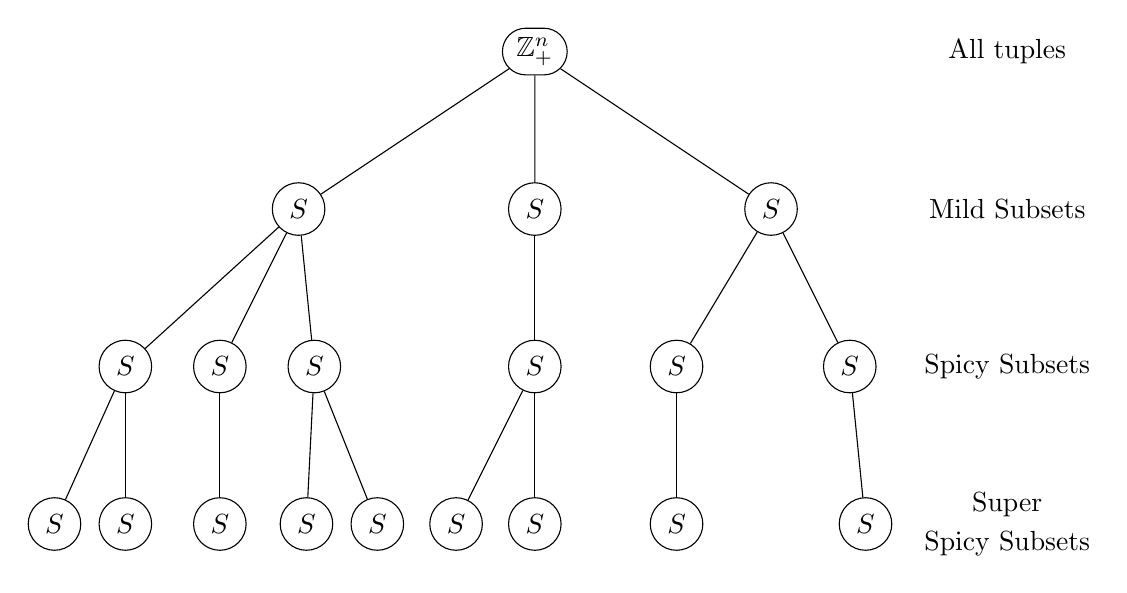
\begin{tikzpicture}
	\node[draw, shape = rounded rectangle] (s0) at (0, 6) {$\mathbb{Z}_+^n $};
	\node[draw, shape = circle] (s1) at (-3, 4) {$ S $};
	\node[draw, shape = circle] (s2) at (0, 4) {$ S $};
	\node[draw, shape = circle] (s3) at (3, 4) {$ S $};

	\node[draw, shape = circle] (s4) at (-5.2, 2) {$ S $};
	\node[draw, shape = circle] (s5) at (-4, 2) {$ S $};
	\node[draw, shape = circle] (s6) at (-2.8, 2) {$ S $};

	\node[draw, shape = circle] (s8) at (0, 2) {$ S $};

	\node[draw, shape = circle] (s10) at (1.8, 2) {$ S $};
	\node[draw, shape = circle] (s12) at (4, 2) {$ S $};

	\node[draw, shape = circle] (s13) at (-6.1, 0) {$ S $};
	\node[draw, shape = circle] (s14) at (-5.2, 0) {$ S $};

	\node[draw, shape = circle] (s15) at (-4, 0) {$ S $};
	\node[draw, shape = circle] (s16) at (-2.9, 0) {$ S $};
	\node[draw, shape = circle] (s17) at (-2, 0) {$ S $};

	\node[draw, shape = circle] (s18) at (-1, 0) {$ S $};
	\node[draw, shape = circle] (s19) at (0, 0) {$ S $};

	\node[draw, shape = circle] (s20) at (1.8, 0) {$ S $};
	\node[draw, shape = circle] (s21) at (4.2, 0) {$ S $};

	\node[] (thing1) at (6,6) {All tuples};
	\node[] (thing1) at (6,4) {Mild Subsets};
	\node[] (thing1) at (6,2) {Spicy Subsets};
	\node[] (thing1) at (6,0.25) {Super};
	\node[] (thing1) at (6,-0.25) {Spicy Subsets};

	\draw
	(s0) edge (s1)
	(s0) edge (s2)
	(s0) edge (s3)

	(s1) edge (s4)
	(s1) edge (s5)
	(s1) edge (s6)

	(s2) edge (s8)

	(s3) edge (s10)
	(s3) edge (s12)

	(s4) edge (s13)
	(s4) edge (s14)

	(s5) edge (s15)

	(s6) edge (s16)
	(s6) edge (s17)

	(s8) edge (s18)
	(s8) edge (s19)

	(s10) edge (s20)
	(s12) edge (s21);

	\end{tikzpicture}
	\caption{Partition Diagram}
\end{figure}
\section{A Multi-layered Partition}
\textbf{Theorem 1.1.} \textit{Two condition codes are equivalent if they are permutations of each other.} \newline
\textbf{Proof.}
Consider any two condition codes \(C_1=(a_1,a_2,...a_n)\) and \(C_2=(b_1,b_2,...b_n)\) which are permutations of each other.
\newline
Assume some \(x \in S(C_1)\).
\newline
By Definition 1.1, a tuple x is an element in \(S(C_1)\) if for all i, there exists a tuple \((t_1,t_2,...t_n)\in \mathbb{Z}_n^+\) such that x contains \(a_i\) copies of \(t_i\). \newline
\newline
Note that a permutation of said tuple \((s_1,s_2,...s_n)\in \mathbb{Z}_n^+\) exists such that for all i, x contains \(b_i\) copies of \(s_i\).
\newline
\newline
Thus, \(x \in S(C_2)\) and \(S(C_2) \subseteq S(C_1)\).
\newline
The same process can be done to show that \(S(C_1) \subseteq S(C_2)\).
\newline
\(\therefore S(C_1) = S(C_2)\) and the condition codes are equivalent.
\newline \(\blacksquare\) \newline \newline
\textbf{Theorem 1.2.} \textit{The set of all spicy subsets S with distinct condition codes C of} \(\mathbb{Z}_n^+\) \textit{forms a disjoint partition of \(\mathbb{Z}_n^+\).} \newline
\textbf{Proof. } Show that each distinct set is disjoint. \newline
Consider any two distinct spicy subsets \(S(C_1)\) and \(S(C_2)\),
where \newline
\(C_1=(a_1,a_2,...a_k),\ C_2=(b_1,b_2,...b_k)\)\newline
Suppose \(x\in S_1\cap S_2\). \newline
\(\exists (t_1,t_2,...t_k) \ni\) x contains \(a_i\) copies of \(t_i\) for all i. \newline
\(\exists (s_1,s_2,..s_k) \ni\) x contains \(b_i\) copies of \(s_i\) for all i.
\newline
This implies that \((t_1,t_2,...t_k)\) is a permutation of \((s_1,s_2,..s_k)\). \newline
This further implies that \(C_1=(a_1,a_2,...a_k),\ C_2=(b_1,b_2,...b_k)\) are permutations of each other and are equivalent by Theorem 1.1.\newline
This is a contradiction. \newline
Thus, there is no \(x \in S_1\cap S_2\).
\newline
\(S_1\cap S_2 = \varnothing\)
\newline \(\square\) \newline
Show that \(\bigcup P =\mathbb{Z}_+^n\). Where P is the set of all spicy subsets.
\newline
\(S\in P \implies S \in \mathbb{Z}_+^n\) by definition. So \(\bigcup P \subseteq \mathbb{Z}_+^n\).
\newline
Assume \(x = (x_1,x_2,...x_n) \in \mathbb{Z}_+^n\).
\newline
Let \(a_i\) be the first occurence of \(x_i\) in x.
\newline
Consider the tuple \((a_1,a_2,...a_k)\) each of whose values are distinct values in x.
\newline
There exists some spicy condition code \(C=(c_1,c_2,...c_k)\) such that x contains \(c_i\) copies of \(a_i\) for all i.
\newline
By Definition 1.2, \(x \in S(C) \in P\) where P is the collection of all spicy subsets.
\newline
by the Union Lemma, \(x \in \bigcup P\)
\newline
\(\mathbb{Z}_+^n \subseteq \bigcup P\)
\newline
\(\therefore \bigcup P = \mathbb{Z}_+^n\)
\newline \(\blacksquare\)

\section{The D function}
\textbf{Definition 1.5.} \textit{Let } \(x = (x_1,x_2,...x_n)\in \mathbb{Z}_+^n\)\textit{ and S(C) be a mild subset or a super spicy subset.}
\newline
\textit{Define }\(D:C\rightarrow \mathbb{R}\) \textit{ by }
\[\sum_{x \in S(C)}\frac{1}{(x_1)^2}\frac{1}{(x_2)^2}...\frac{1}{(x_n)^2}=\sum_{x \in S(C)}\prod_{x_i}x_i^{-2}\]
\textit{For a mild condition code we write: }\(D(c_1)(c_2)...(c_n)\)
\newline
\textit{For a super spicy condition code we write: }\(D(c_1,c_2...c_n)\)
\newline \newline
\textbf{Theorem 1.3} \textit{Let } \(C\) \textit{ be a mild condition code and } \(P\) \textit{ be the collection of all super spicy condition codes } \(C_i\) \textit{ which are subsets of }\(C\).\textit{ Then } \[D(C)=\sum_{C_i\in P}D(C_i)\]
\textbf{Proof. }
\newline
\(\mathbb{Z}_+^n\) has a disjoint parition into super spicy subsets by Theorem 1.2. \newline
Since all super spicy subsets are subsets of mild subsets, every spicy subset has a dijoint partion into super spicy subsets.
\newline
The sum over any set is always equal to the sum over each subset of a disjoint partition.
\newline
Let \(x = (x_1,x_2,...x_n)\in \mathbb{Z}_+^n\), \(C\) be a mild condition code, and each \(C_k\) be super spicy condition codes.
\[\sum_{x \in S(C)}\prod_{x_i}x_i^{-2}=\sum_{S(C_k)\subseteq S(C)}\sum_{x \in S(C_k)}\prod_{x_i}x_i^{-2}\]
\[\therefore D(C)=\sum_{C_i\in P}D(C_i)\]
\(\blacksquare\) \newline
\textbf{Definition 1.6} \newline
\textit{The shorthand for writing } \(D(a,a,a...a)\) \textit{with n} a\textit{s is } \(D_n(a)\).
\newline
\textit{The shorthand for writing } \(D(a)(a)(a)...(a)\) \textit{with n} a\textit{s is } \(D^n(a)\).
\newline
\newline
\textbf{Theorem 1.5} \(D(a)D(b) = D(a)(b)\ \forall a,b\in \mathbb{Z}_+\)
\newline
\textbf{Proof.} By the
\newline
\newline
\textbf{Theorem 1.6} \(D_n(1)=\frac{\pi^{2n}}{(2n+1)!}\)
\newline
\textbf{Proof.}\
We start by comparing the MacLaurin series of \(\sinh(x)\) with the Euler product of \(\sinh(x)\).
\[\sinh(x)=\frac{x}{1!} + \frac{x^3}{3!} + \frac{x^5}{5!} + \frac{x^7}{7!}... =x\left(1+\frac{x}{i\pi}\right)\left(1-\frac{x}{i\pi}\right)\left(1+\frac{x}{2i\pi}\right)\left(1-\frac{x}{2i\pi}\right)...\]
Thus, by a simple calculation,
\[\frac{\sinh(\pi x)}{x}=1+\frac{\pi^2x^2}{3!}+\frac{\pi^4x^4}{5!}+\frac{\pi^6x^6}{7!}...=\left(1+\frac{x^2}{1^2}\right)\left(1+\frac{x^2}{2^2}\right)\left(1+\frac{x^2}{3^2}\right)...\]
\newline
When multiplying a product, to calculate the coefficient on a polynomial of the nth degree, all term combinations resulting in the nth degree of each factor must be determined and subsequently summed. \newline
\newline
For the product expansion, the only term combinations resulting in degree 2 are when we select one \(x^2\) term from one factor and select a 1 from each of the other factors. Comparing this to the right hand side we have
\[\frac{\pi^2}{3!}=\frac{1}{1^2}+\frac{1}{2^2}+\frac{1}{3^2}+\frac{1}{4^2}...=D(1)\]
\newline
\newline
Continuing this process we find that
\[\sum_i\sum_{j<i}\frac{1}{i^2}\frac{1}{j^2}=\frac{\pi^4}{5!}=D(1,1)\]
And in general,
\[\sum_{0<x_1}\sum_{x_2<x_1}...\sum_{x_n<x_{n-1}}\frac{1}{x_1^2}\frac{1}{x_2^2}...\frac{1}{x_n^2}=\frac{\pi^{2n}}{(2n+1)!}=D_n(1)\]
\(\blacksquare\)
\section{References}
\(\ \)
\newline
“Growth and Change in Mathematics.” Understanding Infinity: the Mathematics of Infinite Processes, by A. Gardiner, Dover Publications, 2002, pp. 19–23.
\newline
\newline
Flammable Maths, "The Basel Problem \& its Alternating Formulation [ The Dirichlet Eta Function ]",\textit{YouTube} video, 15:12. Jan. 11, 2019. \newline
https://www.youtube.com/watch?v=MAoI\_\_hbdWM
\newline
\newline
Flammable Maths, "\textbf{BUT HOW DID EULER DO IT}?! A BEAUTIFUL Solution to the FAMOUS Basel Problem!",\textit{YouTube} video, 18:04. May 24, 2019. https://www.youtube.com/watch?v=JAr512hLsEU
\end{document}
